\chapter[PWM Generation and Demodulation]{PWM Generation and Demodulation}

\section*{Aim}

To set-up and implement circuit to carry out pulse width modulation. To design demodulating circuit to detect the message from pulse width modulated wave.
\section*{Theory}
In pulse width modulation method, the width of a constant amplitude constant frequency(constant period T) pulse is varied in accordance with the amplitude of analog modulating signal as shown. Before and after modulation, the amplitude and frequency of the carrier remain constant. Only the pulse width or duty cycle is varying.

Waveforms showing pulse carriers whose width is modulated by message is shown in Figure  \ref{pwmckt}.

Modulation can be carried out using a 555 timer IC configured in monostable multivibrator mode. Normally in a mostable multivibrator the width of the pulse is determined by the time constant of the circuit and the period is determined by the trigger signal period. The width of the pulse is also influneced by the voltage at the control pin-5 of 555 timer IC.  Applying the modulating message signal at pin-5 allows to vary the pulse width as per the modulating signal. 

The demodulation of PWM waveform can be implemented by using a lowpass filter which passes message signal frequenies but blocks the carrier signal.

%\begin{figure}[h]
%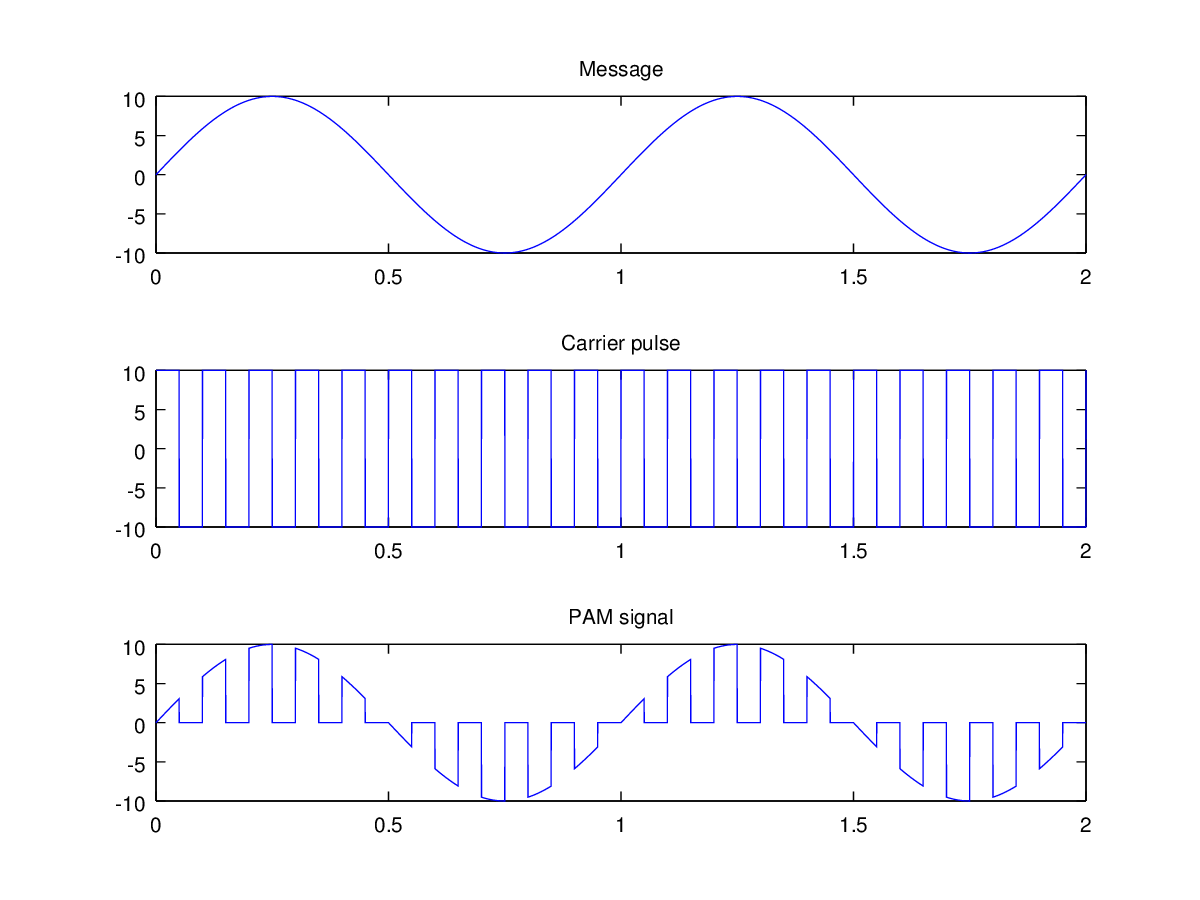
\includegraphics[width=\textwidth]{pam1.png}
%\caption{PAM modulation using transistor}
%\label{PAMmod1}
%\end{figure}
%
%\begin{figure}[h]
%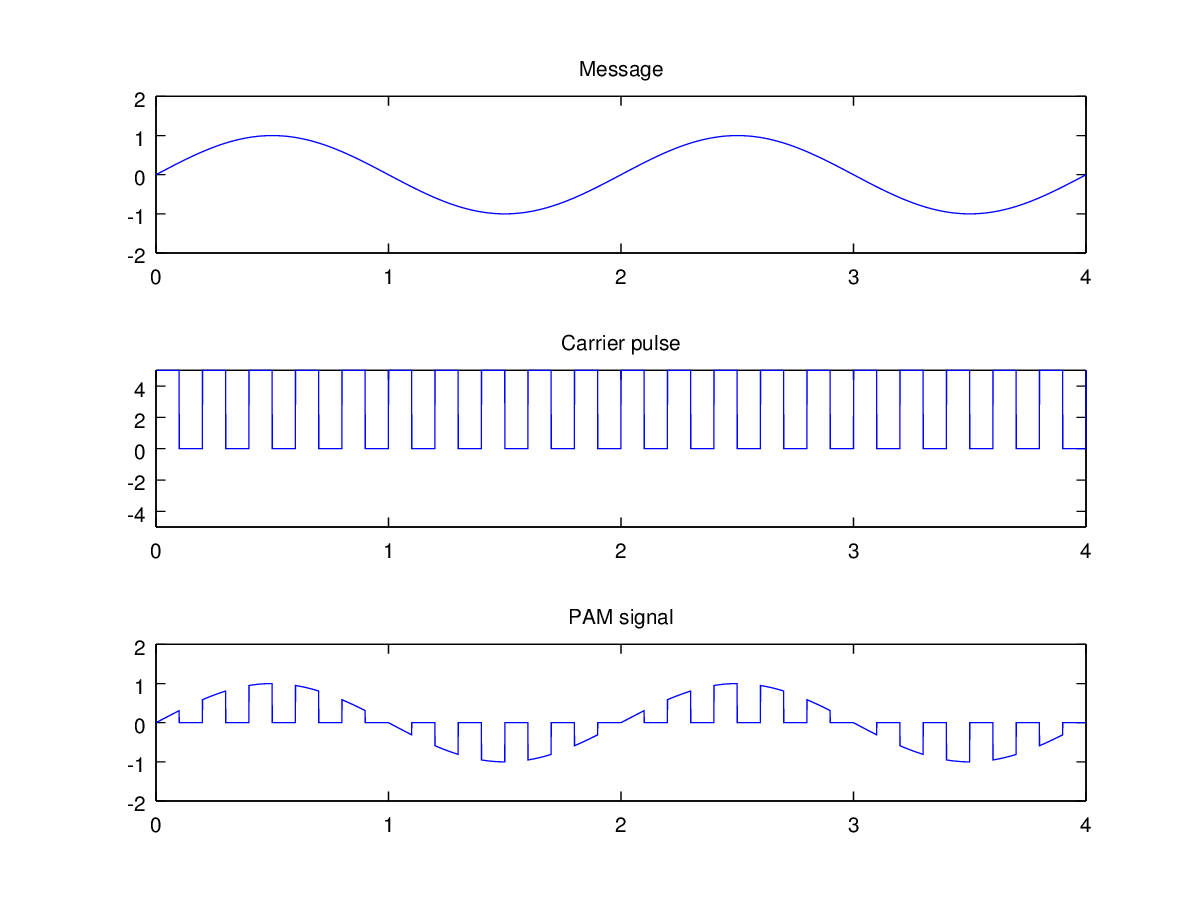
\includegraphics[width=\textwidth]{pam2.png}
%\caption{PAM modulation using switching IC}
%\label{PAMmod2}
%\end{figure}

\section*{Design}
\subsection*{Modulation}

One technique to implement PWM is to use 555 timer IC in monostable multivibrator mode. Without any input signal at control terminal pin-5, the output pulse width is determined by the equation 

\begin{equation}
t_w = 1.1 R C
\end{equation}

This pulse width has to be less than the trigger signal period(T), for the output frequency to be same as the trigger signal frequency.  For a PWM generator to have maximum swing of pulse width for a sinewave modulating signal at pin-5, keep $t_w=\frac{T}{2}$. 

\noindent Select a sampling frequency = Carrier frequency =Trigger signal frequency =5 kHz. ie.,

\begin{equation}
T = 0.2 ms
\end{equation}

\noindent Without modulating signal ($V_C = 0$), the width of the pulse is $t_w=\frac{T}{2}$.

\begin{equation}
t_w=1.1 RC = 0.1 ms
\end{equation}

Assume $C=0.01 \mu F$. Then  $R= 9k\Omega \approx 8.2 k\Omega std	$ (You can use  $C=0.02 \mu F$ and $R=4.7k\Omega$ as well for the same pulse width. )

The modulating signal given must have an amplitude $\le 8 V_{pp}$ ($\le \frac{2V_{CC}}{3}$).

\subsection*{Demodulation}
Demodulation is done using a  $\pi$ RC filter.
\noindent Design the filter as per the equation for upper cut-off frequency of a low pass filter,
\begin{equation}
f_H=\frac{1}{2\pi R_dC_d}
\end{equation}
\noindent Eliminate the high frequency carrier and obtain the low frequency modulating signal from PWM output.

\begin{equation}
1\ kHz=\frac{1}{2\pi R_dC_d}
\end{equation}
\noindent Select $C_d=\ 0.01 \mu F$. Then $R_d \approx 15k\Omega$.
%Choose $R_d=\ 10k\Omega$ standard resistor value.\\

\section*{Circuit Diagram}

The circuit diagram for implementing PWM modulator using 555 IC and demodulation using RC filter is shown.

\begin{figure}
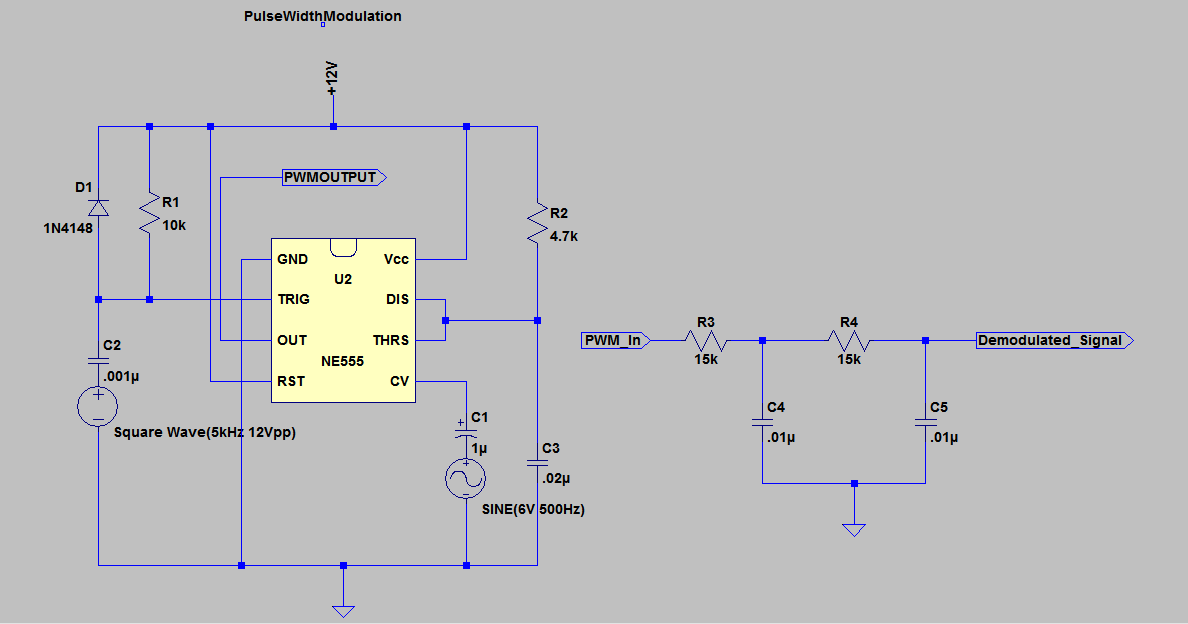
\includegraphics[height= 8cm, width=\textwidth]{pwmckt.png}
\caption{PWM generation and demodulation circuuit}
\label{pwmckt}
\end{figure}




%\section*{Components and Equipments Required}
%CRO (1), \\Signal generator(2),
%\\Resistors: $15\ k\Omega$(2), $10\ k\Omega$(1)
%\\Capacitors: $0.01\  \mu F$(2)
\section*{Procedure}
\begin{itemize}
\item
Connect the PWM generating circuit as shown in the circuit diagram, Figure \ref{pwmckt}.
\item
Feed the carrier pulse (square wave of $5 kHz$, $12V_{PP}$) from the function generator. 
\item
Without applying the modulating signal, see the output waveform at pin-3. It should have 50\% duty cycle. 
\item
Feed the modulating message signal($500 Hz$, $\le 8 V_{pp}$) at pin-5 .
\item
Observe the output on a CRO and plot the graphs of the input and output waveforms.
\item
Make the demodulating circuit as shown in the circuit diagram, Figure \ref{pwmckt}.
\item
Observe the input and output waveforms from PWM demodulation circuit. 
\end{itemize}
\section*{Observation}
Plot the graphs of input and output waveforms as observed on a CRO.
\section*{Result}

Implemented the PWM generation and demodulation circuits and plotted the waveforms.